\artikel{Politik an der Uni?}
{Politik gibt es nicht nur in der großen Welt, sondern auch an Hochschulen. Hier ein kleiner Überblick, welche Gremien wofür stehen und was sie leisten.
}{
    \noindent\textbf{Universitätswahl}\\
    Wie in der Bundes- und Landespolitik auch, hängt der Erfolg der Hochschulpolitik entschieden davon ab, dass sich Leute daran beteiligen.\\
    Dies kannst du auf 2 verschiedenen Wegen tun: Entweder du engagierst dich selbst in den Gremien, oder du nutzt einfach die jährlichen Hochschulwahlen im Sommersemester um deiner Stimme Ausdruck zu verleihen.\\
    Aber warum wählen? Die Wahl ist deine Möglichkeit, in die Hochschulpolitik einzugreifen und etwas zu verändern. Mit deiner Stimmabgabe wählst du dabei nicht nur eine Liste oder Person, du unterstützt auch alle anderen, die dich in diesem Gremium vertreten; denn es ist ein Unterschied, ob die Vertreterinnen und Vertreter von fünf Prozent der Studierenden gewählt wurden oder eben von 50 Prozent.

    Es gibt also mehr als einen guten Grund, zur Wahl zu gehen. Dennoch haben wir in den letzten sechs Jahren ausbaufähige Teilnahmezahlen gehabt. Hier die Wahlbeteiligung der letzten Wahlen:\\

    \begin{tabular}{ll}
        2019 & 12,8\% \\
        2018 & 11,9\% \\
        2017 & 16,9\% \\
        2016 & 15,2\% \\
        2015 & 13,5\% \\
        2014 & 17,9\% \\
    \end{tabular}
    \\\\
    Es waren immer relativ niedrige Ergebnisse, deswegen ist es besonders wichtig, dass du dich an der Wahl beteiligst. Wir werden früh genug darauf aufmerksam machen, sodass du sie nicht verpassen wirst.

    \noindent
    \subsection*{Gremien am Fachbereich:}
    \textbf{Fachbereichsrat}\\
    Der Fachbereichsrat, meist nur FBR genannt, ist das höchste Gremium am Fachbereich. Er behandelt Angelegenheiten von grundsätzlicher Bedeutung für den Fachbereich. Der FBR ist zuständig für

    \begin{itemize}
        \item Erlass der Ordnungen der Studiengänge
        \item Planung der Lehrveranstaltungen
        \item Zusammensetzung von Berufungskommissionen für neue Professor*innen
        \item Ausstattung der Fachgebiete
        \item Abstimmung der Forschungsvorhaben
        \item Wahl des Dekans bzw. der Dekanin
    \end{itemize}

    Dem FBR Informatik gehören sieben Professor*innen, zwei WiMis (Wissenschaftliche Mitarbeiter*innen), ein*e administrativ-technische*r Mitarbeiter*in und drei Studierende an. Gewählt werden diese von ihren jeweiligen Gruppen.

    Wir haben zwar keine Mehrheit, aber das bedeutet nicht, dass wir keinen Einfluss in diesem Gremium hätten. \\

    \noindent\textbf{Fachschaftsrat}

    Der Fachschaftsrat (FSR) besteht nur aus Studierenden und ist so etwas wie die "`gewählte Fachschaft"'. An unserem Fachbereich sind das 9 Personen, doch wir machen keinen wirklichen Unterschied zwischen gewählten Fachschaftler*innen und solchen, die sich einfach so beteiligen wollen. Jede*r ist herzlich dazu eingeladen, mitzuarbeiten.\\

    Die Fachschaft vertritt die Interessen aller Informatikstudierenden und setzt sich stetig dafür ein, das Informatikstudium an der TU noch besser zu machen. Dazu trifft sich die Fachschaft normalerweise zu wöchentlichen Sitzungen (derzeit Mittwochs um 18:00 Uhr) und in verschiedenen Arbeitskreisen und Ausschüssen. Wir entsenden außerdem Leute zur Fachschaftenkonferenz, wo einmal im Monat Probleme zwischen allen Fachschaften der TU geklärt werden, und zur KIF, der Konferenz der deutschsprachigen Informatikfachschaften.\\

    Sie ist außerdem Ansprechpartnerin bei Fragen und Problemen rund um das Studium. Auch Probleme mit Professor*innen können hier durchaus angesprochen werden.

    Mehr zur Fachschaft und zum Fachschaftsrat findest du im Artikel "`Fragen und Antworten rund ums Thema Fachschaft"', oder du besuchst uns einfach mal in Raum D120.

    \subsection*{Uniweite Gremien:}
    \noindent\textbf{Universitätsversammlung}

    In der Universitätsversammlung (UV) sind die Studierenden mit 15 Mitgliedern vertreten. Ihnen stehen 31 Professor*innen, zehn wissenschaftliche Mitarbeiter*innen und  fünf administrativ-technische Mitarbeiter*innen aller Fachbereiche gegenüber.

    \noindent Wie bei allen universitätsweiten Gremien gibt es hier Listenwahl, keine Personenwahl. Auf jeder Liste stehen Vertreterinnen und Vertreter verschiedener Fachbereiche, einige Listen verfolgen die Ziele ihrer "`großen Mutterparteien"', andere dagegen sind unabhängig.

    Die Aufgaben der UV sind die Wahl des Präsidiums und die Verabschiedung von Ordnungen, die die ganze Universität betreffen. Außerdem wählt sie die Mitglieder des Senats, darunter befinden sich auch vier studentische.\\

    \noindent\textbf{Studierendenparlament}

    Das Studierendenparlament (StuPa) besteht aus 31 studentischen Mitgliedern, die per Listenwahl gewählt werden. Seine Aufgabe ist vor allem die Wahl und Kontrolle des Allgemeinen Studierendenausschusses (AStA) sowie Verwaltung des Haushaltes der Studierendenschaft.\\

    \noindent\textbf{Senat}

    Der Senat der TU Darmstadt überwacht die Geschäftsführung des Präsidiums und berät es in Angelegenheiten, die die Struktur, die Entwicklungs- und Bauplanung, den Haushalt, die Forschung, die Lehre oder das Studium betreffen. Der Senat hat 20 Mitglieder, die von der Universitätsversammlung gewählt werden. Unter ihnen sind vier Studierende.\\

    \noindent\textbf{AStA}

    Der Allgemeine Studierendenaussschuss (AStA) ist die Vertretung der Studierenden auf Hochschulebene und wird größtenteils vom Studierendenparlament gewählt.
    Auf politischer Ebene setzt sich der AStA für die Interessen aller Studierenden ein und ist außerdem verantwortlich für eine Vielzahl an Serviceangeboten.
    Mehr über den AStA erfährt du im nächsten Artikel.

}
{Julian Haas}

\bildmitunterschrift{comics/two_party_system}{width=\textwidth}{}{xkcd.com}

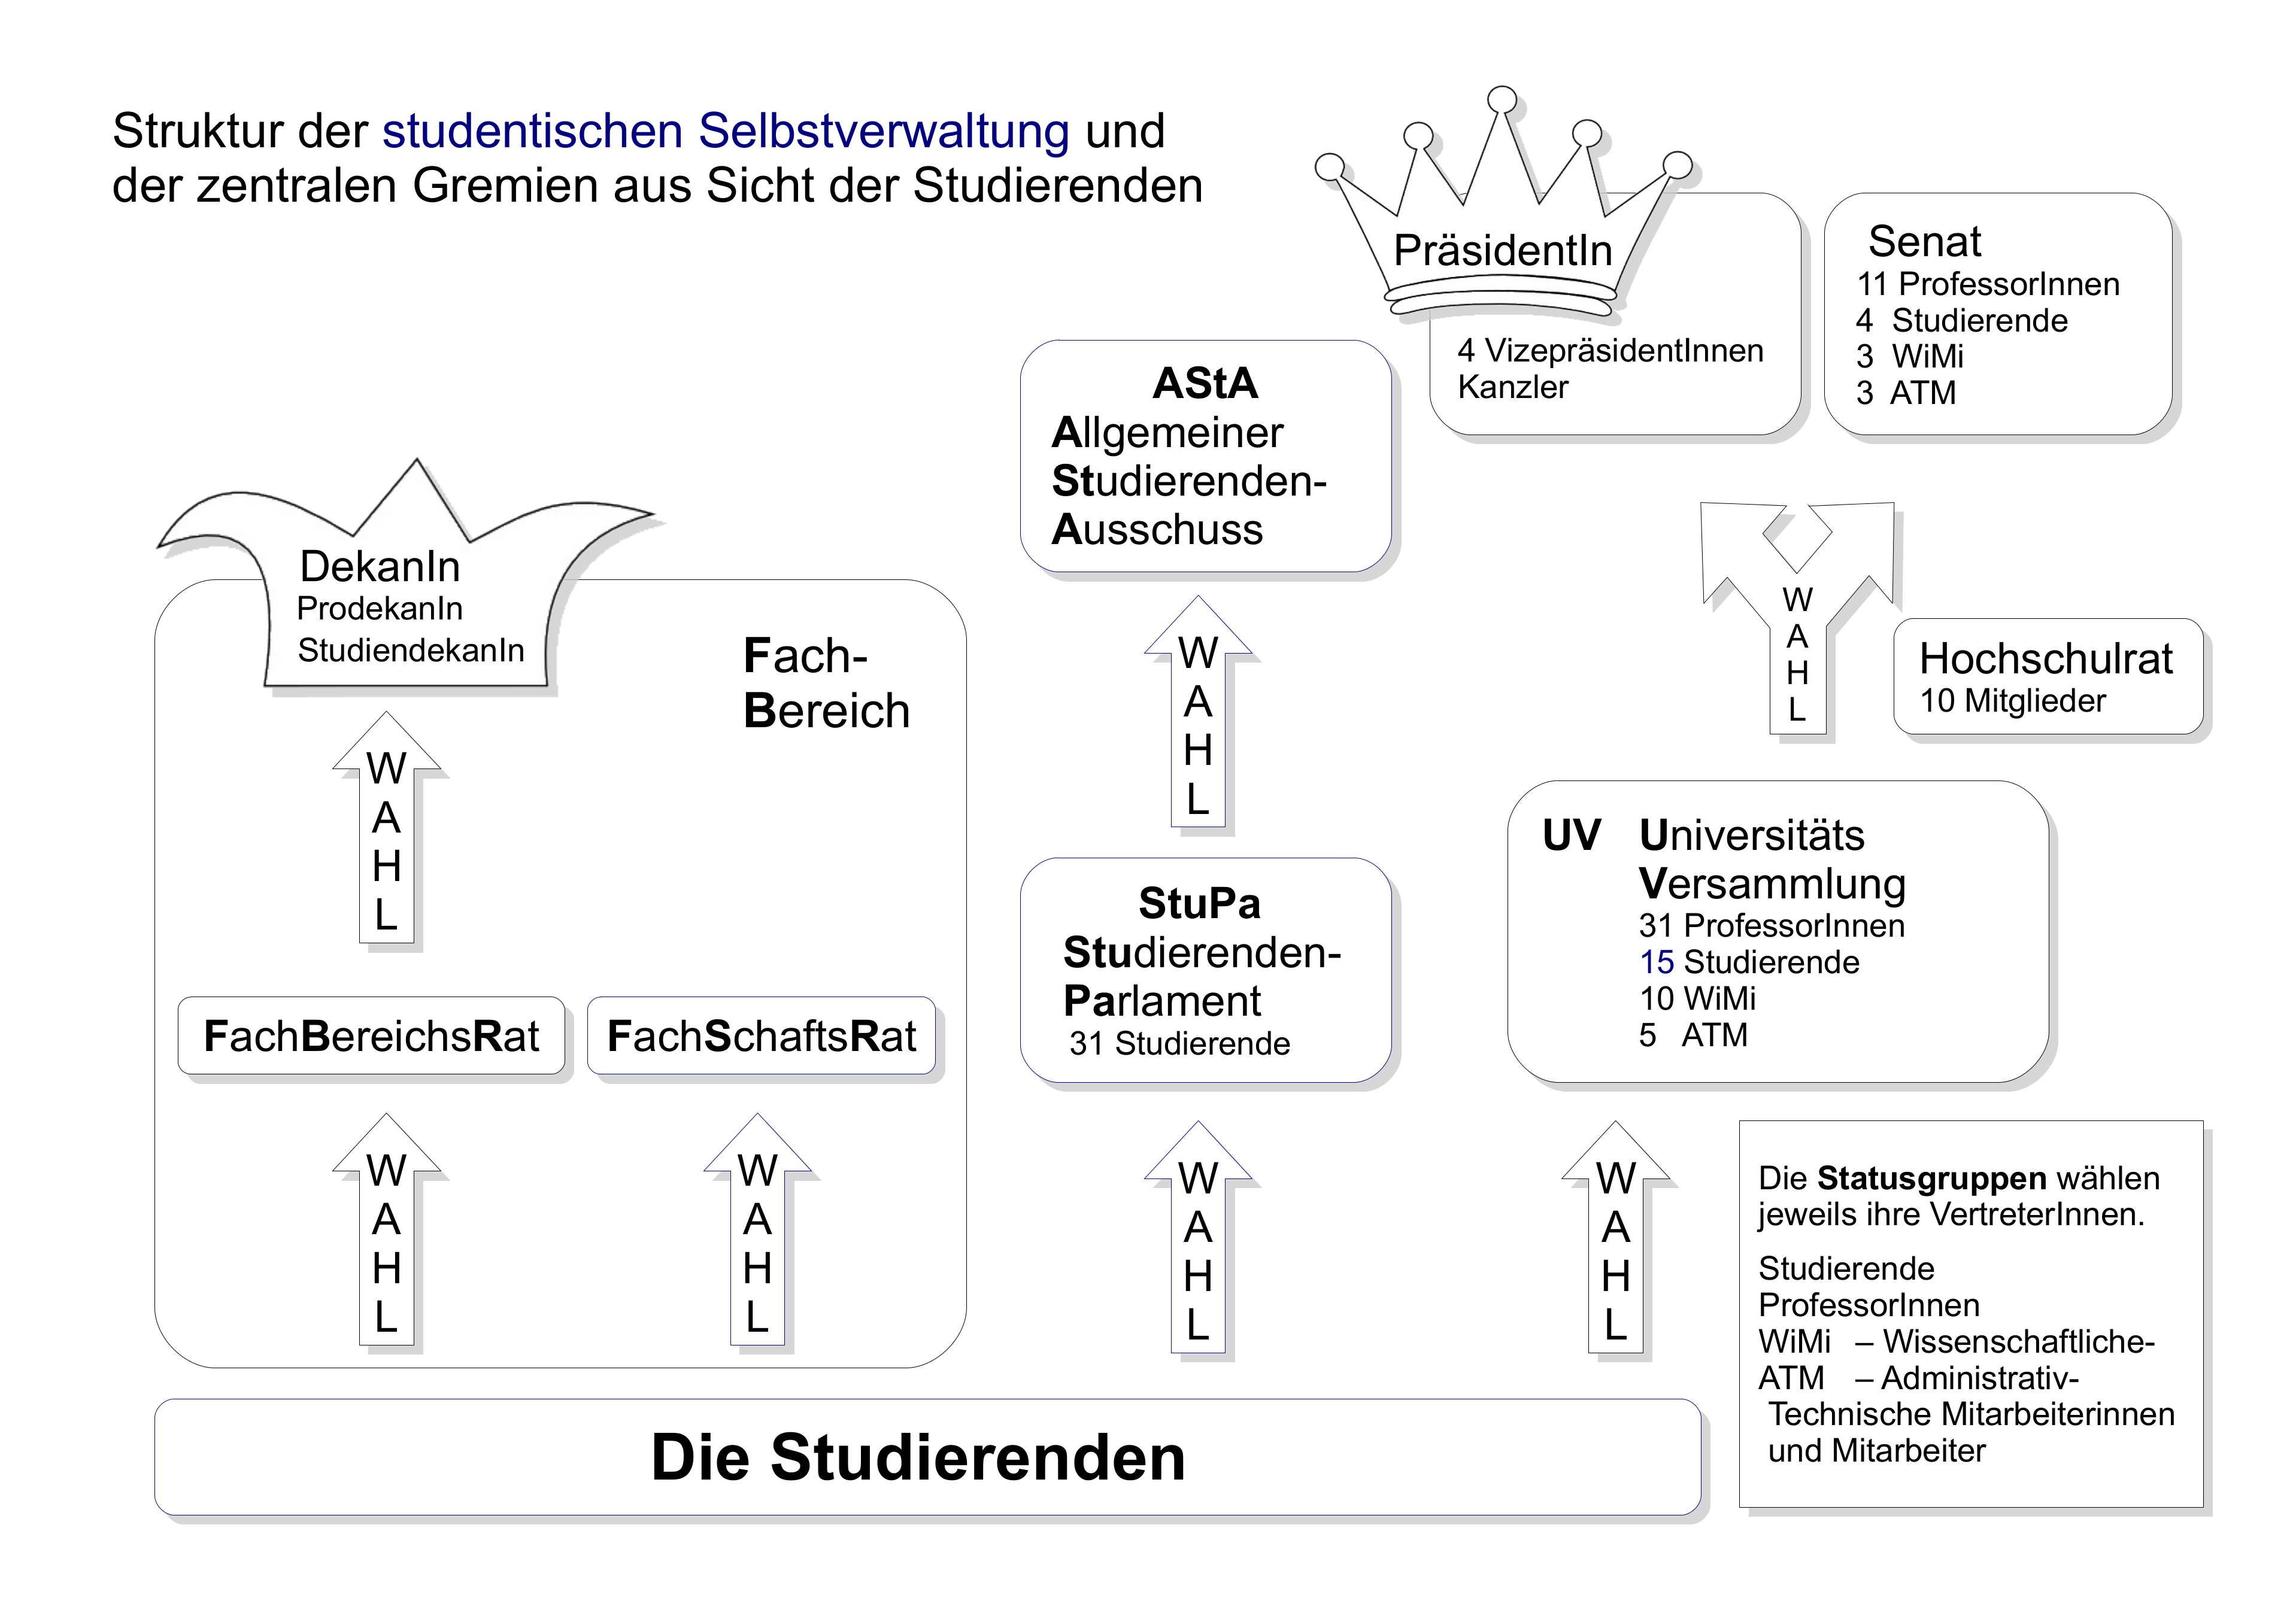
\includegraphics[angle=270,totalheight=17cm]{artikel/hopo2}

\newpage
